% Options for packages loaded elsewhere
\PassOptionsToPackage{unicode}{hyperref}
\PassOptionsToPackage{hyphens}{url}
%
\documentclass[
]{article}
\usepackage{amsmath,amssymb}
\usepackage{lmodern}
\usepackage{iftex}
\ifPDFTeX
  \usepackage[T1]{fontenc}
  \usepackage[utf8]{inputenc}
  \usepackage{textcomp} % provide euro and other symbols
\else % if luatex or xetex
  \usepackage{unicode-math}
  \defaultfontfeatures{Scale=MatchLowercase}
  \defaultfontfeatures[\rmfamily]{Ligatures=TeX,Scale=1}
\fi
% Use upquote if available, for straight quotes in verbatim environments
\IfFileExists{upquote.sty}{\usepackage{upquote}}{}
\IfFileExists{microtype.sty}{% use microtype if available
  \usepackage[]{microtype}
  \UseMicrotypeSet[protrusion]{basicmath} % disable protrusion for tt fonts
}{}
\makeatletter
\@ifundefined{KOMAClassName}{% if non-KOMA class
  \IfFileExists{parskip.sty}{%
    \usepackage{parskip}
  }{% else
    \setlength{\parindent}{0pt}
    \setlength{\parskip}{6pt plus 2pt minus 1pt}}
}{% if KOMA class
  \KOMAoptions{parskip=half}}
\makeatother
\usepackage{xcolor}
\IfFileExists{xurl.sty}{\usepackage{xurl}}{} % add URL line breaks if available
\IfFileExists{bookmark.sty}{\usepackage{bookmark}}{\usepackage{hyperref}}
\hypersetup{
  hidelinks,
  pdfcreator={LaTeX via pandoc}}
\urlstyle{same} % disable monospaced font for URLs
\usepackage[margin=1in]{geometry}
\usepackage{color}
\usepackage{fancyvrb}
\newcommand{\VerbBar}{|}
\newcommand{\VERB}{\Verb[commandchars=\\\{\}]}
\DefineVerbatimEnvironment{Highlighting}{Verbatim}{commandchars=\\\{\}}
% Add ',fontsize=\small' for more characters per line
\usepackage{framed}
\definecolor{shadecolor}{RGB}{248,248,248}
\newenvironment{Shaded}{\begin{snugshade}}{\end{snugshade}}
\newcommand{\AlertTok}[1]{\textcolor[rgb]{0.94,0.16,0.16}{#1}}
\newcommand{\AnnotationTok}[1]{\textcolor[rgb]{0.56,0.35,0.01}{\textbf{\textit{#1}}}}
\newcommand{\AttributeTok}[1]{\textcolor[rgb]{0.77,0.63,0.00}{#1}}
\newcommand{\BaseNTok}[1]{\textcolor[rgb]{0.00,0.00,0.81}{#1}}
\newcommand{\BuiltInTok}[1]{#1}
\newcommand{\CharTok}[1]{\textcolor[rgb]{0.31,0.60,0.02}{#1}}
\newcommand{\CommentTok}[1]{\textcolor[rgb]{0.56,0.35,0.01}{\textit{#1}}}
\newcommand{\CommentVarTok}[1]{\textcolor[rgb]{0.56,0.35,0.01}{\textbf{\textit{#1}}}}
\newcommand{\ConstantTok}[1]{\textcolor[rgb]{0.00,0.00,0.00}{#1}}
\newcommand{\ControlFlowTok}[1]{\textcolor[rgb]{0.13,0.29,0.53}{\textbf{#1}}}
\newcommand{\DataTypeTok}[1]{\textcolor[rgb]{0.13,0.29,0.53}{#1}}
\newcommand{\DecValTok}[1]{\textcolor[rgb]{0.00,0.00,0.81}{#1}}
\newcommand{\DocumentationTok}[1]{\textcolor[rgb]{0.56,0.35,0.01}{\textbf{\textit{#1}}}}
\newcommand{\ErrorTok}[1]{\textcolor[rgb]{0.64,0.00,0.00}{\textbf{#1}}}
\newcommand{\ExtensionTok}[1]{#1}
\newcommand{\FloatTok}[1]{\textcolor[rgb]{0.00,0.00,0.81}{#1}}
\newcommand{\FunctionTok}[1]{\textcolor[rgb]{0.00,0.00,0.00}{#1}}
\newcommand{\ImportTok}[1]{#1}
\newcommand{\InformationTok}[1]{\textcolor[rgb]{0.56,0.35,0.01}{\textbf{\textit{#1}}}}
\newcommand{\KeywordTok}[1]{\textcolor[rgb]{0.13,0.29,0.53}{\textbf{#1}}}
\newcommand{\NormalTok}[1]{#1}
\newcommand{\OperatorTok}[1]{\textcolor[rgb]{0.81,0.36,0.00}{\textbf{#1}}}
\newcommand{\OtherTok}[1]{\textcolor[rgb]{0.56,0.35,0.01}{#1}}
\newcommand{\PreprocessorTok}[1]{\textcolor[rgb]{0.56,0.35,0.01}{\textit{#1}}}
\newcommand{\RegionMarkerTok}[1]{#1}
\newcommand{\SpecialCharTok}[1]{\textcolor[rgb]{0.00,0.00,0.00}{#1}}
\newcommand{\SpecialStringTok}[1]{\textcolor[rgb]{0.31,0.60,0.02}{#1}}
\newcommand{\StringTok}[1]{\textcolor[rgb]{0.31,0.60,0.02}{#1}}
\newcommand{\VariableTok}[1]{\textcolor[rgb]{0.00,0.00,0.00}{#1}}
\newcommand{\VerbatimStringTok}[1]{\textcolor[rgb]{0.31,0.60,0.02}{#1}}
\newcommand{\WarningTok}[1]{\textcolor[rgb]{0.56,0.35,0.01}{\textbf{\textit{#1}}}}
\usepackage{longtable,booktabs,array}
\usepackage{calc} % for calculating minipage widths
% Correct order of tables after \paragraph or \subparagraph
\usepackage{etoolbox}
\makeatletter
\patchcmd\longtable{\par}{\if@noskipsec\mbox{}\fi\par}{}{}
\makeatother
% Allow footnotes in longtable head/foot
\IfFileExists{footnotehyper.sty}{\usepackage{footnotehyper}}{\usepackage{footnote}}
\makesavenoteenv{longtable}
\usepackage{graphicx}
\makeatletter
\def\maxwidth{\ifdim\Gin@nat@width>\linewidth\linewidth\else\Gin@nat@width\fi}
\def\maxheight{\ifdim\Gin@nat@height>\textheight\textheight\else\Gin@nat@height\fi}
\makeatother
% Scale images if necessary, so that they will not overflow the page
% margins by default, and it is still possible to overwrite the defaults
% using explicit options in \includegraphics[width, height, ...]{}
\setkeys{Gin}{width=\maxwidth,height=\maxheight,keepaspectratio}
% Set default figure placement to htbp
\makeatletter
\def\fps@figure{htbp}
\makeatother
\setlength{\emergencystretch}{3em} % prevent overfull lines
\providecommand{\tightlist}{%
  \setlength{\itemsep}{0pt}\setlength{\parskip}{0pt}}
\setcounter{secnumdepth}{-\maxdimen} % remove section numbering
\newlength{\cslhangindent}
\setlength{\cslhangindent}{1.5em}
\newlength{\csllabelwidth}
\setlength{\csllabelwidth}{3em}
\newlength{\cslentryspacingunit} % times entry-spacing
\setlength{\cslentryspacingunit}{\parskip}
\newenvironment{CSLReferences}[2] % #1 hanging-ident, #2 entry spacing
 {% don't indent paragraphs
  \setlength{\parindent}{0pt}
  % turn on hanging indent if param 1 is 1
  \ifodd #1
  \let\oldpar\par
  \def\par{\hangindent=\cslhangindent\oldpar}
  \fi
  % set entry spacing
  \setlength{\parskip}{#2\cslentryspacingunit}
 }%
 {}
\usepackage{calc}
\newcommand{\CSLBlock}[1]{#1\hfill\break}
\newcommand{\CSLLeftMargin}[1]{\parbox[t]{\csllabelwidth}{#1}}
\newcommand{\CSLRightInline}[1]{\parbox[t]{\linewidth - \csllabelwidth}{#1}\break}
\newcommand{\CSLIndent}[1]{\hspace{\cslhangindent}#1}
\usepackage{float}
\ifLuaTeX
  \usepackage{selnolig}  % disable illegal ligatures
\fi

\author{}
\date{\vspace{-2.5em}}

\begin{document}

Diagnosis plots for all the statistical models used in ``Impact of cropping system diversification on vegetative and reproductive characteristics of waterhemp (Amaranthus tuberculatus)'' with \texttt{ggResidpanel} (Goode and Rey 2019).

\hypertarget{crop-yield-at-the-experiment-site}{%
\paragraph*{Crop yield at the experiment site}\label{crop-yield-at-the-experiment-site}}
\addcontentsline{toc}{paragraph}{Crop yield at the experiment site}

Crop identity in these yield models represented rotation system (2-year, 3-year or 4-year) for corn and soybean or 3-year and 4-year for oat.

\begin{Shaded}
\begin{Highlighting}[]
\DocumentationTok{\#\# Did crop identity and corn weed management affect corn yield?}

\NormalTok{corn.lmer }\OtherTok{\textless{}{-}} \FunctionTok{lmer}\NormalTok{(}\FunctionTok{log}\NormalTok{(Standardized\_yield\_MgpHa) }\SpecialCharTok{\textasciitilde{}}\NormalTok{ Block }\SpecialCharTok{+} 
\NormalTok{                    Crop\_ID}\SpecialCharTok{*}\NormalTok{Corn\_weed\_management }\SpecialCharTok{+} 
\NormalTok{                    (}\DecValTok{1}\SpecialCharTok{|}\NormalTok{Year) }\SpecialCharTok{+}
\NormalTok{                    (}\DecValTok{1}\SpecialCharTok{|}\NormalTok{Year}\SpecialCharTok{:}\NormalTok{Block) }\SpecialCharTok{+} 
\NormalTok{                    (}\DecValTok{1}\SpecialCharTok{|}\NormalTok{Year}\SpecialCharTok{:}\NormalTok{Crop\_ID) }\SpecialCharTok{+} 
\NormalTok{                    (}\DecValTok{1}\SpecialCharTok{|}\NormalTok{Year}\SpecialCharTok{:}\NormalTok{Corn\_weed\_management) }\SpecialCharTok{+} 
\NormalTok{                    (}\DecValTok{1}\SpecialCharTok{|}\NormalTok{Year}\SpecialCharTok{:}\NormalTok{Crop\_ID}\SpecialCharTok{:}\NormalTok{Corn\_weed\_management)  }\SpecialCharTok{+}
\NormalTok{                    (}\DecValTok{1}\SpecialCharTok{|}\NormalTok{Block}\SpecialCharTok{:}\NormalTok{Year}\SpecialCharTok{:}\NormalTok{Crop\_ID) ,}
  \AttributeTok{data=}\NormalTok{corn) }\CommentTok{\#corn was harvested on hafl{-}plot basis}

\FunctionTok{resid\_panel}\NormalTok{(corn.lmer, }\StringTok{"all"}\NormalTok{)}
\end{Highlighting}
\end{Shaded}

\begin{figure}
\centering
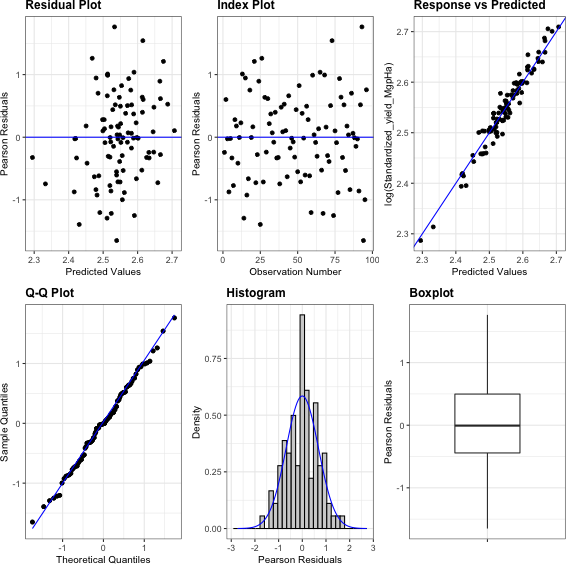
\includegraphics{AppendixA-model-diagnosis_files/figure-latex/corn-mod-1.png}
\caption{\label{fig:corn-mod}Diagnosis plot for the effect of crop identity and corn weed management on corn yield over four years with four blocks of replication.}
\end{figure}

\begin{Shaded}
\begin{Highlighting}[]
\DocumentationTok{\#\# Did crop identity and corn weed management affect soybean yield?}

\NormalTok{soy.lmer }\OtherTok{\textless{}{-}} \FunctionTok{lmer}\NormalTok{(}\FunctionTok{log}\NormalTok{(Standardized\_yield\_MgpHa) }\SpecialCharTok{\textasciitilde{}}\NormalTok{ Block }\SpecialCharTok{+} 
\NormalTok{                   Crop\_ID}\SpecialCharTok{*}\NormalTok{Corn\_weed\_management }\SpecialCharTok{+} 
\NormalTok{                   (}\DecValTok{1}\SpecialCharTok{|}\NormalTok{Year) }\SpecialCharTok{+} 
\NormalTok{                   (}\DecValTok{1}\SpecialCharTok{|}\NormalTok{Year}\SpecialCharTok{:}\NormalTok{Block) }\SpecialCharTok{+} 
\NormalTok{                   (}\DecValTok{1}\SpecialCharTok{|}\NormalTok{Year}\SpecialCharTok{:}\NormalTok{Crop\_ID) }\SpecialCharTok{+} 
\NormalTok{                   (}\DecValTok{1}\SpecialCharTok{|}\NormalTok{Year}\SpecialCharTok{:}\NormalTok{Corn\_weed\_management) }\SpecialCharTok{+}
\NormalTok{                   (}\DecValTok{1}\SpecialCharTok{|}\NormalTok{Year}\SpecialCharTok{:}\NormalTok{Crop\_ID}\SpecialCharTok{:}\NormalTok{Corn\_weed\_management)  }\SpecialCharTok{+} 
\NormalTok{                   (}\DecValTok{1}\SpecialCharTok{|}\NormalTok{Block}\SpecialCharTok{:}\NormalTok{Year}\SpecialCharTok{:}\NormalTok{Crop\_ID),}
  \AttributeTok{data=}\NormalTok{soy) }\CommentTok{\#soybean was harvested on hafl{-}plot basis}

\FunctionTok{resid\_panel}\NormalTok{(soy.lmer, }\StringTok{"all"}\NormalTok{)}
\end{Highlighting}
\end{Shaded}

\begin{figure}
\centering
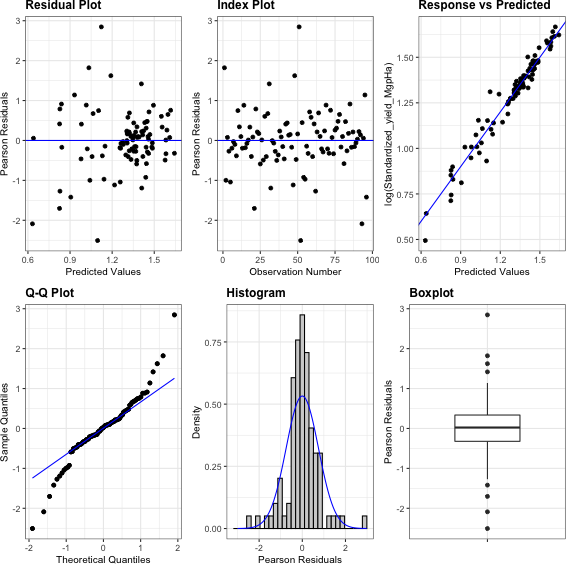
\includegraphics{AppendixA-model-diagnosis_files/figure-latex/soy-mod-1.png}
\caption{\label{fig:soy-mod}Diagnosis plot for the effect of crop identity and corn weed management on soybean yield over four years with four blocks of replication.}
\end{figure}

\begin{Shaded}
\begin{Highlighting}[]
\DocumentationTok{\#\# Did crop identity affect oat yield?}
\CommentTok{\# crop identity represented rotation system (3{-}year or 4{-}year)}

\NormalTok{oat.lmer }\OtherTok{\textless{}{-}} \FunctionTok{lmer}\NormalTok{(}\FunctionTok{log}\NormalTok{(Standardized\_yield\_MgpHa) }\SpecialCharTok{\textasciitilde{}}\NormalTok{ Block }\SpecialCharTok{+} 
\NormalTok{                   Crop\_ID }\SpecialCharTok{+} 
\NormalTok{                   (}\DecValTok{1}\SpecialCharTok{|}\NormalTok{Year) }\SpecialCharTok{+}
\NormalTok{                   (}\DecValTok{1}\SpecialCharTok{|}\NormalTok{Year}\SpecialCharTok{:}\NormalTok{Block) }\SpecialCharTok{+}  
\NormalTok{                   (}\DecValTok{1}\SpecialCharTok{|}\NormalTok{Year}\SpecialCharTok{:}\NormalTok{Crop\_ID) }\SpecialCharTok{+}
\NormalTok{                   (}\DecValTok{1}\SpecialCharTok{|}\NormalTok{Block}\SpecialCharTok{:}\NormalTok{Year}\SpecialCharTok{:}\NormalTok{Crop\_ID),}
  \AttributeTok{data=}\NormalTok{oat) }\CommentTok{\#oat was harvested in whol{-}plot basis }

\FunctionTok{resid\_panel}\NormalTok{(oat.lmer, }\StringTok{"all"}\NormalTok{)}
\end{Highlighting}
\end{Shaded}

\begin{figure}
\centering
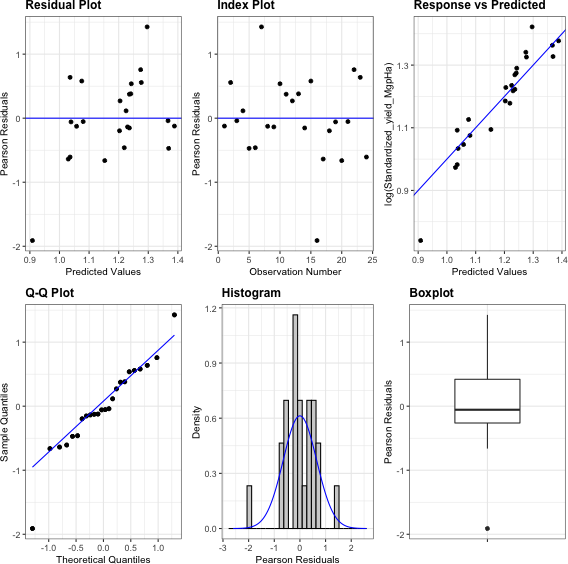
\includegraphics{AppendixA-model-diagnosis_files/figure-latex/oat-mod-1.png}
\caption{\label{fig:oat-mod}Diagnosis plot for the effect of crop identity on oat yield over four years with four blocks of replication.}
\end{figure}

\hypertarget{community-ecological-indices}{%
\paragraph*{Community ecological indices}\label{community-ecological-indices}}
\addcontentsline{toc}{paragraph}{Community ecological indices}

Crop identities in these ecological indices models were the combinations of the crop species names' one-letter abbreviation and the rotation to which the crop belonged.

\begin{Shaded}
\begin{Highlighting}[]
\DocumentationTok{\#\# Did crop identity and corn weed management affect weed community diversity index?}

\NormalTok{dens\_diversity.lmer1 }\OtherTok{\textless{}{-}} \FunctionTok{lmer}\NormalTok{(}\FunctionTok{log}\NormalTok{(Diversity }\SpecialCharTok{+} \DecValTok{1}\NormalTok{) }\SpecialCharTok{\textasciitilde{}}\NormalTok{ Block }\SpecialCharTok{+} 
\NormalTok{                               Crop\_ID}\SpecialCharTok{*}\NormalTok{Corn\_weed\_management }\SpecialCharTok{+} 
\NormalTok{                               (}\DecValTok{1}\SpecialCharTok{|}\NormalTok{Year) }\SpecialCharTok{+}\NormalTok{ (}\DecValTok{1}\SpecialCharTok{|}\NormalTok{Year}\SpecialCharTok{:}\NormalTok{Block) }\SpecialCharTok{+} 
\NormalTok{                               (}\DecValTok{1}\SpecialCharTok{|}\NormalTok{Year}\SpecialCharTok{:}\NormalTok{Crop\_ID) }\SpecialCharTok{+} 
\NormalTok{                               (}\DecValTok{1}\SpecialCharTok{|}\NormalTok{Year}\SpecialCharTok{:}\NormalTok{Corn\_weed\_management) }\SpecialCharTok{+}
\NormalTok{                               (}\DecValTok{1}\SpecialCharTok{|}\NormalTok{Year}\SpecialCharTok{:}\NormalTok{Crop\_ID}\SpecialCharTok{:}\NormalTok{Corn\_weed\_management)  }\SpecialCharTok{+}
\NormalTok{                               (}\DecValTok{1}\SpecialCharTok{|}\NormalTok{Block}\SpecialCharTok{:}\NormalTok{Year}\SpecialCharTok{:}\NormalTok{Crop\_ID) , }
                   \AttributeTok{data =}\NormalTok{ dens\_ind\_1720,}
                   \AttributeTok{control=}\FunctionTok{lmerControl}\NormalTok{(}\AttributeTok{check.conv.singular =} \FunctionTok{.makeCC}\NormalTok{(}\AttributeTok{action =} \StringTok{"ignore"}\NormalTok{,  }\AttributeTok{tol =} \FloatTok{1e{-}4}\NormalTok{))) }
\CommentTok{\# summary(dens\_diversity.lmer1)$sigma \#0.27}
\FunctionTok{resid\_panel}\NormalTok{(dens\_diversity.lmer1, }\StringTok{"all"}\NormalTok{)}
\end{Highlighting}
\end{Shaded}

\begin{figure}
\centering
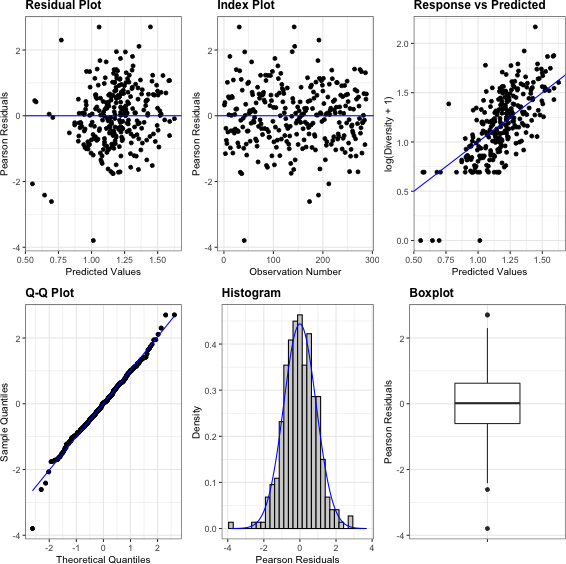
\includegraphics{AppendixA-model-diagnosis_files/figure-latex/dens-div-mod-1.png}
\caption{\label{fig:dens-div-mod}Diagnosis plot for the effect of crop identity and corn weed management on weed community density diversity index over four years with four blocks of replication.}
\end{figure}

\begin{Shaded}
\begin{Highlighting}[]
\DocumentationTok{\#\# Did crop identity and corn weed management affect weed community evenness index?}

\CommentTok{\#min(dens\_ind\_1720$Evenness[dens\_ind\_1720$Evenness \textgreater{} 0])  \#0.016156463}
\NormalTok{dens\_even.lmer4 }\OtherTok{\textless{}{-}} \FunctionTok{lmer}\NormalTok{(}\FunctionTok{log}\NormalTok{(Evenness }\SpecialCharTok{+} \FloatTok{0.016156463}\NormalTok{) }\SpecialCharTok{\textasciitilde{}}\NormalTok{  Block }\SpecialCharTok{+} 
\NormalTok{                          Crop\_ID }\SpecialCharTok{*}\NormalTok{ Corn\_weed\_management }\SpecialCharTok{+} 
\NormalTok{                          (}\DecValTok{1}\SpecialCharTok{|}\NormalTok{Year) }\SpecialCharTok{+} 
\NormalTok{                          (}\DecValTok{1}\SpecialCharTok{|}\NormalTok{Year}\SpecialCharTok{:}\NormalTok{Block) }\SpecialCharTok{+} 
\NormalTok{                          (}\DecValTok{1}\SpecialCharTok{|}\NormalTok{Year}\SpecialCharTok{:}\NormalTok{Crop\_ID) }\SpecialCharTok{+}
\NormalTok{                          (}\DecValTok{1}\SpecialCharTok{|}\NormalTok{Year}\SpecialCharTok{:}\NormalTok{Corn\_weed\_management) }\SpecialCharTok{+}
\NormalTok{                          (}\DecValTok{1}\SpecialCharTok{|}\NormalTok{Year}\SpecialCharTok{:}\NormalTok{Crop\_ID}\SpecialCharTok{:}\NormalTok{Corn\_weed\_management)  }\SpecialCharTok{+}
\NormalTok{                          (}\DecValTok{1}\SpecialCharTok{|}\NormalTok{Block}\SpecialCharTok{:}\NormalTok{Year}\SpecialCharTok{:}\NormalTok{Crop\_ID) , }
                   \AttributeTok{data =}\NormalTok{ dens\_ind\_1720,}
                   \AttributeTok{control=}\FunctionTok{lmerControl}\NormalTok{(}\AttributeTok{check.conv.singular =} \FunctionTok{.makeCC}\NormalTok{(}\AttributeTok{action =} \StringTok{"ignore"}\NormalTok{,  }\AttributeTok{tol =} \FloatTok{1e{-}4}\NormalTok{))) }
\CommentTok{\#summary(dens\_even.lmer4)$sigma \# 0.68 \# second best sigma, better than arcsin sqrt transform and more spread out points}

\FunctionTok{resid\_panel}\NormalTok{(dens\_even.lmer4, }\StringTok{"all"}\NormalTok{)}
\end{Highlighting}
\end{Shaded}

\begin{figure}
\centering
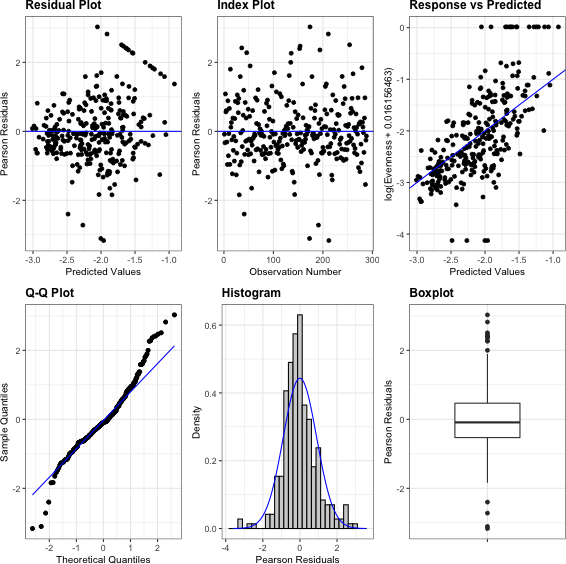
\includegraphics{AppendixA-model-diagnosis_files/figure-latex/dens-even-mod-1.png}
\caption{\label{fig:dens-even-mod}Diagnosis plot for the effect of crop identity and corn weed management on weed community density evenness index over four years with four blocks of replication.}
\end{figure}

\begin{Shaded}
\begin{Highlighting}[]
\DocumentationTok{\#\# Did crop identity and corn weed management affect weed community density richness index?  }

\NormalTok{dens\_rich.lmer2 }\OtherTok{\textless{}{-}} \FunctionTok{lmer}\NormalTok{(}\FunctionTok{log}\NormalTok{(Richness}\SpecialCharTok{+}\DecValTok{1}\NormalTok{) }\SpecialCharTok{\textasciitilde{}}\NormalTok{ Block }\SpecialCharTok{+} 
\NormalTok{                          Crop\_ID }\SpecialCharTok{*}\NormalTok{ Corn\_weed\_management }\SpecialCharTok{+} 
\NormalTok{                          (}\DecValTok{1}\SpecialCharTok{|}\NormalTok{Year) }\SpecialCharTok{+}
\NormalTok{                          (}\DecValTok{1}\SpecialCharTok{|}\NormalTok{Year}\SpecialCharTok{:}\NormalTok{Block) }\SpecialCharTok{+} 
\NormalTok{                          (}\DecValTok{1}\SpecialCharTok{|}\NormalTok{Year}\SpecialCharTok{:}\NormalTok{Crop\_ID) }\SpecialCharTok{+}
\NormalTok{                         (}\DecValTok{1}\SpecialCharTok{|}\NormalTok{Year}\SpecialCharTok{:}\NormalTok{Corn\_weed\_management) }\SpecialCharTok{+} 
\NormalTok{                       (}\DecValTok{1}\SpecialCharTok{|}\NormalTok{Year}\SpecialCharTok{:}\NormalTok{Crop\_ID}\SpecialCharTok{:}\NormalTok{Corn\_weed\_management) }\SpecialCharTok{+} 
\NormalTok{                         (}\DecValTok{1}\SpecialCharTok{|}\NormalTok{Block}\SpecialCharTok{:}\NormalTok{Year}\SpecialCharTok{:}\NormalTok{Crop\_ID) , }
                   \AttributeTok{data =}\NormalTok{ dens\_ind\_1720, }
                   \AttributeTok{control=}\FunctionTok{lmerControl}\NormalTok{(}\AttributeTok{check.conv.singular =} \FunctionTok{.makeCC}\NormalTok{(}\AttributeTok{action =} \StringTok{"ignore"}\NormalTok{,  }\AttributeTok{tol =} \FloatTok{1e{-}4}\NormalTok{))) }
\CommentTok{\# summary(dens\_rich.lmer2)$sigma  \#0.288}
\FunctionTok{resid\_panel}\NormalTok{(dens\_rich.lmer2, }\StringTok{"all"}\NormalTok{ )}
\end{Highlighting}
\end{Shaded}

\begin{figure}
\centering
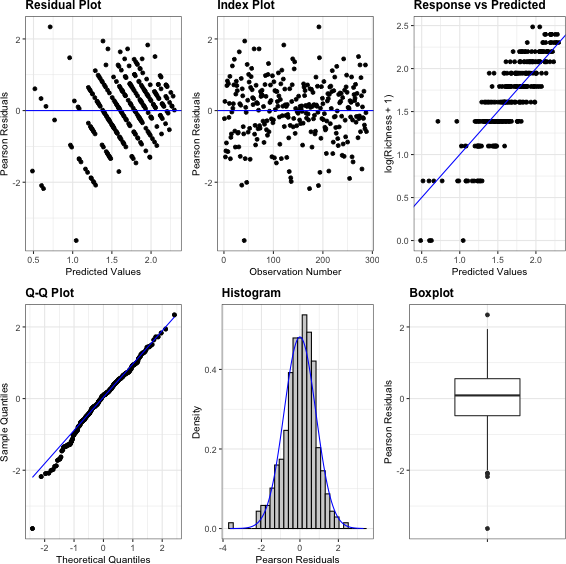
\includegraphics{AppendixA-model-diagnosis_files/figure-latex/dens-rich-mod-1.png}
\caption{\label{fig:dens-rich-mod}Diagnosis plot for the effect of crop identity and corn weed management on weed community density richness index over four years with four blocks of replication.}
\end{figure}

\begin{Shaded}
\begin{Highlighting}[]
\DocumentationTok{\#\# Did crop identity and corn weed management affect weed community biomass diversity index?}

\CommentTok{\# min(biom\_ind\_1720$Diversity[biom\_ind\_1720$Diversity \textgreater{} 0])}
\NormalTok{biom\_diversity.lmer1 }\OtherTok{\textless{}{-}} \FunctionTok{lmer}\NormalTok{(}\FunctionTok{log}\NormalTok{(Diversity }\SpecialCharTok{+} \DecValTok{1}\NormalTok{ ) }\SpecialCharTok{\textasciitilde{}}\NormalTok{  Block }\SpecialCharTok{+} 
\NormalTok{                               Crop\_ID }\SpecialCharTok{*}\NormalTok{ Corn\_weed\_management }\SpecialCharTok{+} 
\NormalTok{                               (}\DecValTok{1}\SpecialCharTok{|}\NormalTok{Year) }\SpecialCharTok{+} 
\NormalTok{                               (}\DecValTok{1}\SpecialCharTok{|}\NormalTok{Block}\SpecialCharTok{:}\NormalTok{Year) }\SpecialCharTok{+} 
\NormalTok{                               (}\DecValTok{1}\SpecialCharTok{|}\NormalTok{Year}\SpecialCharTok{:}\NormalTok{Crop\_ID) }\SpecialCharTok{+} 
\NormalTok{                               (}\DecValTok{1}\SpecialCharTok{|}\NormalTok{Year}\SpecialCharTok{:}\NormalTok{Corn\_weed\_management) }\SpecialCharTok{+} 
\NormalTok{                               (}\DecValTok{1}\SpecialCharTok{|}\NormalTok{Year}\SpecialCharTok{:}\NormalTok{Crop\_ID}\SpecialCharTok{:}\NormalTok{Corn\_weed\_management)  }\SpecialCharTok{+} 
\NormalTok{                               (}\DecValTok{1}\SpecialCharTok{|}\NormalTok{Block}\SpecialCharTok{:}\NormalTok{Year}\SpecialCharTok{:}\NormalTok{Crop\_ID)  , }
                   \AttributeTok{data =}\NormalTok{ biom\_ind\_1720,}
                   \AttributeTok{control=}\FunctionTok{lmerControl}\NormalTok{(}\AttributeTok{check.conv.singular =} \FunctionTok{.makeCC}\NormalTok{(}\AttributeTok{action =} \StringTok{"ignore"}\NormalTok{,  }\AttributeTok{tol =} \FloatTok{1e{-}4}\NormalTok{))) }
\CommentTok{\# summary(biom\_diversity.lmer1)$sigma \#0.25}

\FunctionTok{resid\_panel}\NormalTok{(biom\_diversity.lmer1, }\StringTok{"all"}\NormalTok{)}
\end{Highlighting}
\end{Shaded}

\begin{figure}
\centering
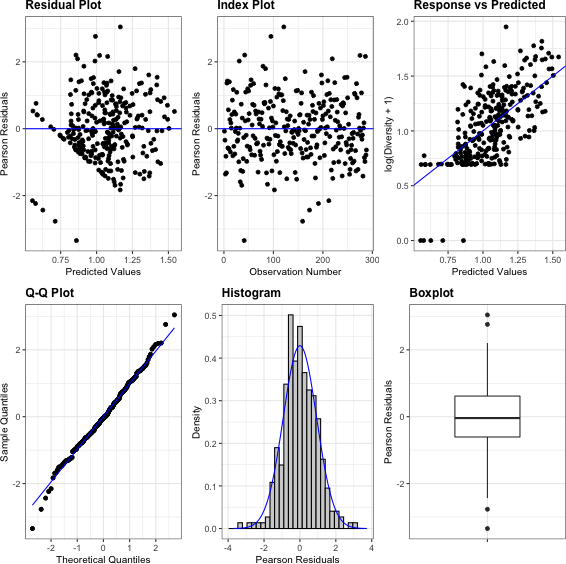
\includegraphics{AppendixA-model-diagnosis_files/figure-latex/biom-div-mod-1.png}
\caption{\label{fig:biom-div-mod}Diagnosis plot for the effect of crop identity and corn weed management on weed community aboveground mass diversity index over four years with four blocks of replication.}
\end{figure}

\begin{Shaded}
\begin{Highlighting}[]
\DocumentationTok{\#\# Did crop identity and corn weed management affect weed community aboveground mass evenness index?}
\FunctionTok{min}\NormalTok{(biom\_ind\_1720}\SpecialCharTok{$}\NormalTok{Evenness[biom\_ind\_1720}\SpecialCharTok{$}\NormalTok{Evenness }\SpecialCharTok{\textgreater{}} \DecValTok{0}\NormalTok{]) }
\end{Highlighting}
\end{Shaded}

\begin{verbatim}
## [1] 0.01510172
\end{verbatim}

\begin{Shaded}
\begin{Highlighting}[]
\NormalTok{biom\_even.lmer4 }\OtherTok{\textless{}{-}} \FunctionTok{lmer}\NormalTok{(}\FunctionTok{log}\NormalTok{(Evenness }\SpecialCharTok{+} \FloatTok{0.015101721}\NormalTok{ ) }\SpecialCharTok{\textasciitilde{}}\NormalTok{ Block }\SpecialCharTok{+} 
\NormalTok{                          Crop\_ID }\SpecialCharTok{*}\NormalTok{ Corn\_weed\_management }\SpecialCharTok{+} 
\NormalTok{                        (}\DecValTok{1}\SpecialCharTok{|}\NormalTok{Year) }\SpecialCharTok{+}\NormalTok{ (}\DecValTok{1}\SpecialCharTok{|}\NormalTok{Year}\SpecialCharTok{:}\NormalTok{Block) }\SpecialCharTok{+} 
\NormalTok{                       (}\DecValTok{1}\SpecialCharTok{|}\NormalTok{Year}\SpecialCharTok{:}\NormalTok{Crop\_ID) }\SpecialCharTok{+}\NormalTok{ (}\DecValTok{1}\SpecialCharTok{|}\NormalTok{Year}\SpecialCharTok{:}\NormalTok{Corn\_weed\_management) }\SpecialCharTok{+} 
\NormalTok{                       (}\DecValTok{1}\SpecialCharTok{|}\NormalTok{Year}\SpecialCharTok{:}\NormalTok{Crop\_ID}\SpecialCharTok{:}\NormalTok{Corn\_weed\_management)  }\SpecialCharTok{+} 
\NormalTok{                         (}\DecValTok{1}\SpecialCharTok{|}\NormalTok{Block}\SpecialCharTok{:}\NormalTok{Year}\SpecialCharTok{:}\NormalTok{Crop\_ID) , }
                   \AttributeTok{data =}\NormalTok{ biom\_ind\_1720,}
                   \AttributeTok{control=}\FunctionTok{lmerControl}\NormalTok{(}\AttributeTok{check.conv.singular =} \FunctionTok{.makeCC}\NormalTok{(}\AttributeTok{action =} \StringTok{"ignore"}\NormalTok{,  }\AttributeTok{tol =} \FloatTok{1e{-}4}\NormalTok{))) }
\CommentTok{\#summary(biom\_even.lmer4)$sigma \# 0.72 \# second best sigma, points more spread{-}out }

\FunctionTok{resid\_panel}\NormalTok{(biom\_even.lmer4, }\StringTok{"all"}\NormalTok{)}
\end{Highlighting}
\end{Shaded}

\begin{figure}
\centering
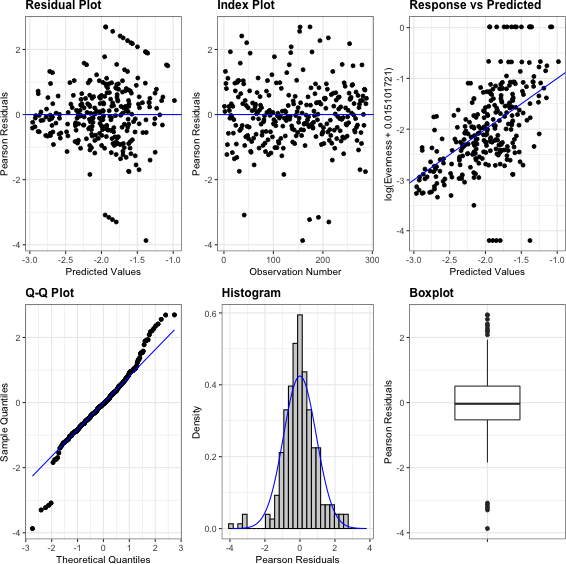
\includegraphics{AppendixA-model-diagnosis_files/figure-latex/biom-even-mod-1.png}
\caption{\label{fig:biom-even-mod}Diagnosis plot for the effect of crop identity and corn weed management on weed community aboveground mass evenness index over four years with four blocks of replication.}
\end{figure}

\begin{Shaded}
\begin{Highlighting}[]
\DocumentationTok{\#\# Did crop identity and corn weed management affect weed community aboveground mass richness index?}

\CommentTok{\# min( biom\_ind\_1720$Richness[ biom\_ind\_1720$Richness \textgreater{} 0])}
\NormalTok{biom\_rich.lmer2 }\OtherTok{\textless{}{-}} \FunctionTok{lmer}\NormalTok{(}\FunctionTok{log}\NormalTok{(Richness }\SpecialCharTok{+} \DecValTok{1}\NormalTok{) }\SpecialCharTok{\textasciitilde{}}\NormalTok{  Block }\SpecialCharTok{+} 
\NormalTok{                          Crop\_ID }\SpecialCharTok{*}\NormalTok{ Corn\_weed\_management }\SpecialCharTok{+} 
\NormalTok{                        (}\DecValTok{1}\SpecialCharTok{|}\NormalTok{Year)  }\SpecialCharTok{+}
\NormalTok{                          (}\DecValTok{1}\SpecialCharTok{|}\NormalTok{Year}\SpecialCharTok{:}\NormalTok{Block) }\SpecialCharTok{+} 
\NormalTok{                       (}\DecValTok{1}\SpecialCharTok{|}\NormalTok{Year}\SpecialCharTok{:}\NormalTok{Crop\_ID) }\SpecialCharTok{+}
\NormalTok{                         (}\DecValTok{1}\SpecialCharTok{|}\NormalTok{Year}\SpecialCharTok{:}\NormalTok{Corn\_weed\_management) }\SpecialCharTok{+} 
\NormalTok{                       (}\DecValTok{1}\SpecialCharTok{|}\NormalTok{Year}\SpecialCharTok{:}\NormalTok{Crop\_ID}\SpecialCharTok{:}\NormalTok{Corn\_weed\_management)  }\SpecialCharTok{+}
\NormalTok{                         (}\DecValTok{1}\SpecialCharTok{|}\NormalTok{Block}\SpecialCharTok{:}\NormalTok{Year}\SpecialCharTok{:}\NormalTok{Crop\_ID) , }
                   \AttributeTok{data =}\NormalTok{ biom\_ind\_1720, }
                   \AttributeTok{control=}\FunctionTok{lmerControl}\NormalTok{(}\AttributeTok{check.conv.singular =} \FunctionTok{.makeCC}\NormalTok{(}\AttributeTok{action =} \StringTok{"ignore"}\NormalTok{,  }\AttributeTok{tol =} \FloatTok{1e{-}4}\NormalTok{))) }

\CommentTok{\#summary(biom\_rich.lmer2)$sigma  \#0.2935}

\FunctionTok{resid\_panel}\NormalTok{(biom\_rich.lmer2 , }\StringTok{"all"}\NormalTok{)}
\end{Highlighting}
\end{Shaded}

\begin{figure}
\centering
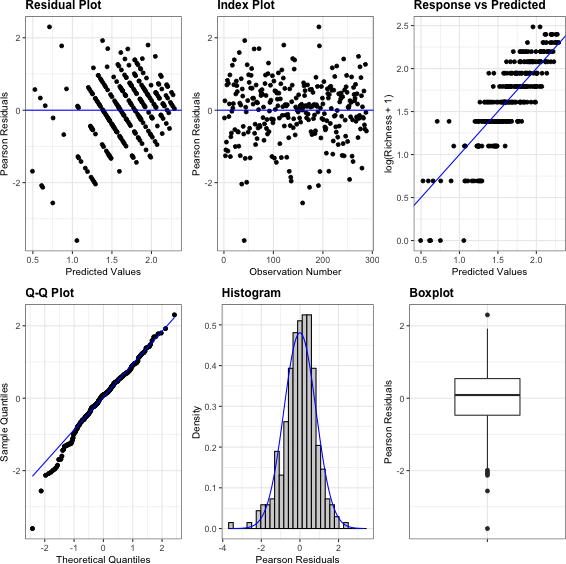
\includegraphics{AppendixA-model-diagnosis_files/figure-latex/biom-rich-mod-1.png}
\caption{\label{fig:biom-rich-mod}Diagnosis plot for the effect of crop identity and corn weed management on weed community aboveground mass richness index over four years with four blocks of replication.}
\end{figure}

\hypertarget{total-weed-community-density-and-aboveground-mass}{%
\paragraph*{Total weed community density and aboveground mass}\label{total-weed-community-density-and-aboveground-mass}}
\addcontentsline{toc}{paragraph}{Total weed community density and aboveground mass}

\begin{figure}
\centering
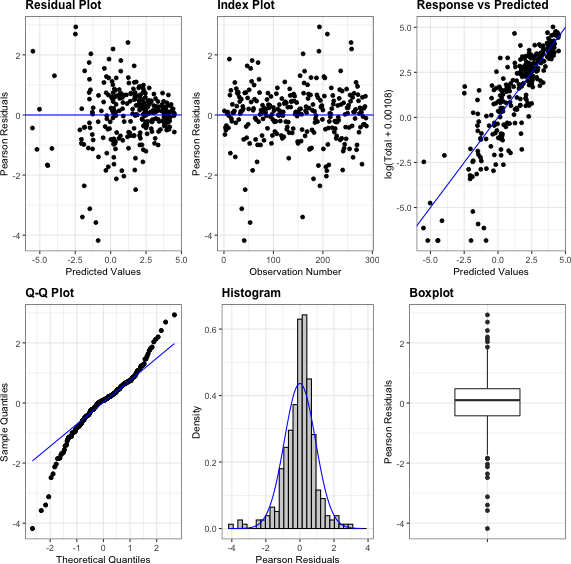
\includegraphics{AppendixA-model-diagnosis_files/figure-latex/all-biom-mod-1.png}
\caption{\label{fig:all-biom-mod}Diagnosis plot for the effect of crop identity and corn weed management on weed community aboveground mass over four years with four blocks of replication.}
\end{figure}

\begin{figure}
\centering
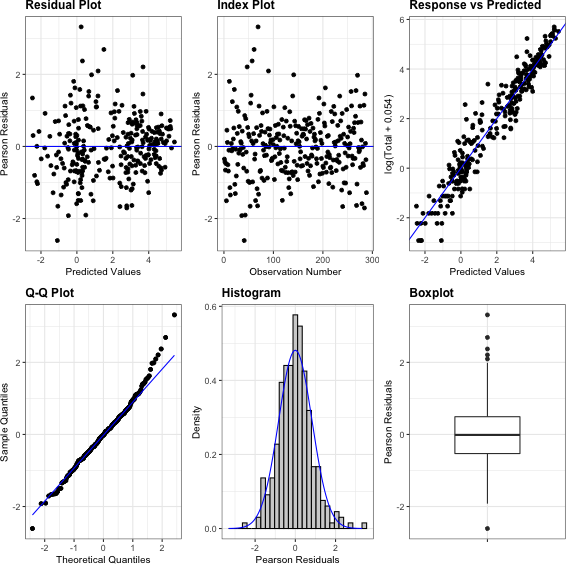
\includegraphics{AppendixA-model-diagnosis_files/figure-latex/all-dens-mod-1.png}
\caption{\label{fig:all-dens-mod}Diagnosis plot for the effect of crop identity and corn weed management on weed community density over four years with four blocks of replication.}
\end{figure}

\hypertarget{top-seven-species-individual-density}{%
\paragraph*{Top seven species individual density}\label{top-seven-species-individual-density}}
\addcontentsline{toc}{paragraph}{Top seven species individual density}

\begin{Shaded}
\begin{Highlighting}[]
\DocumentationTok{\#\#\#\#\# Fit all species at once with split{-}fit{-}combine syntax }
\CommentTok{\# https://stat585{-}at{-}isu.github.io/materials{-}2019/04\_functional{-}programming/02\_purrr.html\#23}


\CommentTok{\# convert wide to long format }

\NormalTok{dens\_1720\_long }\OtherTok{\textless{}{-}}\NormalTok{ dens\_1720\_clean }\SpecialCharTok{\%\textgreater{}\%} 
  \FunctionTok{pivot\_longer}\NormalTok{(}\SpecialCharTok{!}\FunctionTok{c}\NormalTok{(Crop}\SpecialCharTok{:}\NormalTok{Corn\_weed\_management), }
               \AttributeTok{names\_to =} \StringTok{"Species"}\NormalTok{, }\AttributeTok{values\_to =}  \StringTok{"Density"}\NormalTok{)}

\CommentTok{\#singularity because of too many zeros in many species columns }


\CommentTok{\# min(dens\_1720\_long$Density[dens\_1720\_long$Density\textgreater{}0]) \#0.05396072}

\NormalTok{dens\_result\_t }\OtherTok{\textless{}{-}}\NormalTok{ dens\_1720\_long }\SpecialCharTok{\%\textgreater{}\%}
  \FunctionTok{group\_by}\NormalTok{(Species) }\SpecialCharTok{\%\textgreater{}\%} 
  \FunctionTok{nest}\NormalTok{() }\SpecialCharTok{\%\textgreater{}\%}
  \FunctionTok{mutate}\NormalTok{(}\AttributeTok{models=}\FunctionTok{map}\NormalTok{(data,}\SpecialCharTok{\textasciitilde{}}\FunctionTok{lmer}\NormalTok{(}\FunctionTok{log}\NormalTok{(Density }\SpecialCharTok{+} \FloatTok{0.05396072}\NormalTok{) }\SpecialCharTok{\textasciitilde{}}\NormalTok{ Block }\SpecialCharTok{+}\NormalTok{ Crop\_ID }\SpecialCharTok{+}
\NormalTok{                                 Corn\_weed\_management  }\SpecialCharTok{+}
\NormalTok{                                 Crop\_ID}\SpecialCharTok{:}\NormalTok{Corn\_weed\_management }\SpecialCharTok{+} 
\NormalTok{                                 (}\DecValTok{1}\SpecialCharTok{|}\NormalTok{Year) }\SpecialCharTok{+}\NormalTok{ (}\DecValTok{1}\SpecialCharTok{|}\NormalTok{Year}\SpecialCharTok{:}\NormalTok{Block) }\SpecialCharTok{+} 
\NormalTok{                                 (}\DecValTok{1}\SpecialCharTok{|}\NormalTok{Year}\SpecialCharTok{:}\NormalTok{Crop\_ID) }\SpecialCharTok{+} 
\NormalTok{                                 (}\DecValTok{1}\SpecialCharTok{|}\NormalTok{Year}\SpecialCharTok{:}\NormalTok{Corn\_weed\_management) }\SpecialCharTok{+} 
\NormalTok{                                 (}\DecValTok{1}\SpecialCharTok{|}\NormalTok{Year}\SpecialCharTok{:}\NormalTok{Crop\_ID}\SpecialCharTok{:}\NormalTok{Corn\_weed\_management)  }\SpecialCharTok{+}
\NormalTok{                                 (}\DecValTok{1}\SpecialCharTok{|}\NormalTok{Block}\SpecialCharTok{:}\NormalTok{Year}\SpecialCharTok{:}\NormalTok{Crop\_ID) ,}\AttributeTok{data =}\NormalTok{.x))) }\SpecialCharTok{\%\textgreater{}\%}
\NormalTok{  ungroup }\SpecialCharTok{\%\textgreater{}\%}
  \FunctionTok{mutate}\NormalTok{(}\AttributeTok{diag\_plots =} \FunctionTok{map}\NormalTok{(models, resid\_panel, }\StringTok{"all"}\NormalTok{),}
    \AttributeTok{jts =} \FunctionTok{map}\NormalTok{(models, joint\_tests),}
         \FunctionTok{across}\NormalTok{(diag\_plots}\SpecialCharTok{:}\NormalTok{jts, setNames,  .}\SpecialCharTok{$}\NormalTok{Species))}
\end{Highlighting}
\end{Shaded}

\begin{figure}
\centering
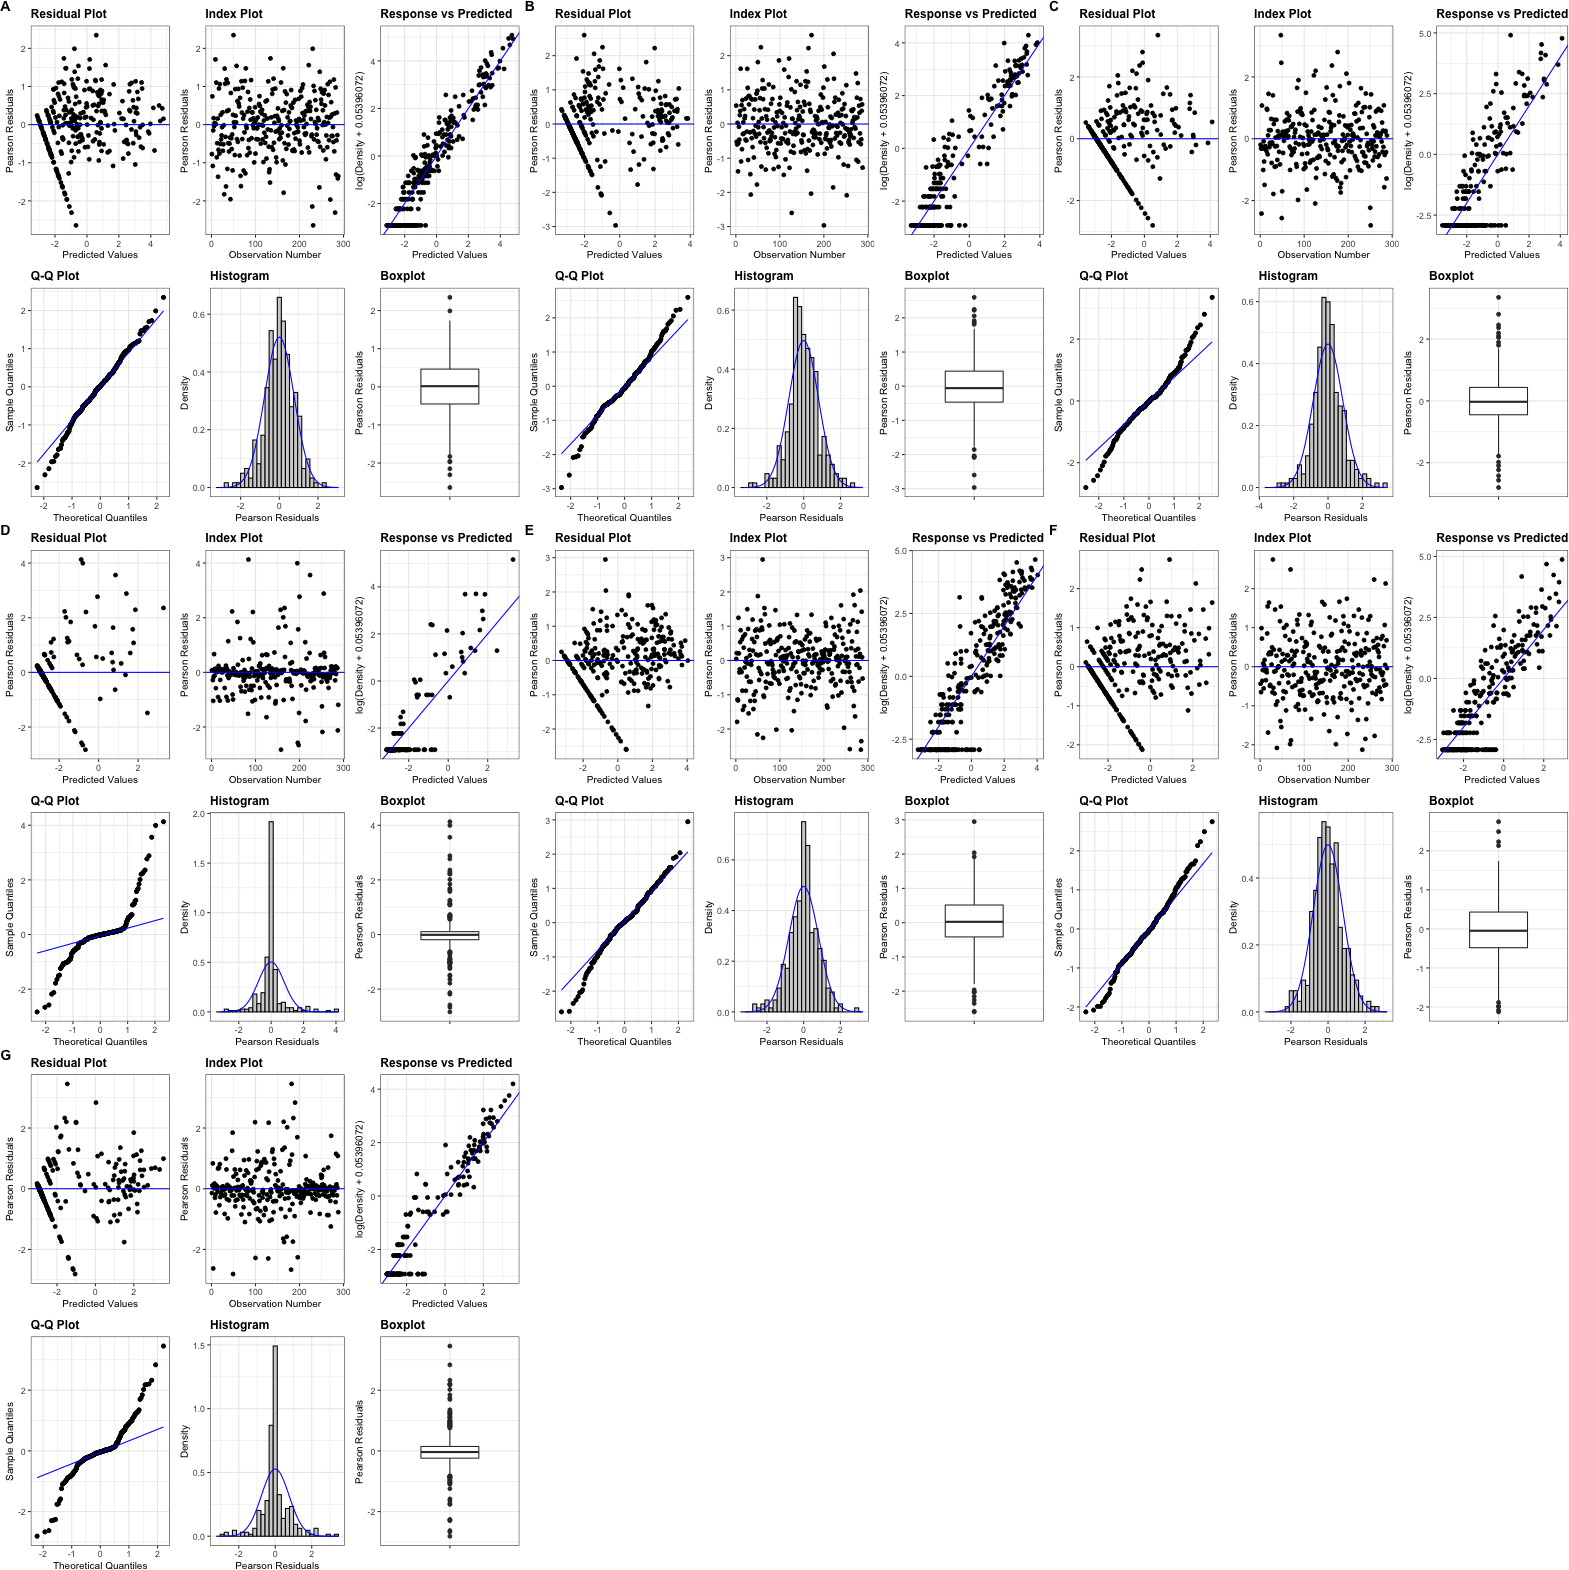
\includegraphics{AppendixA-model-diagnosis_files/figure-latex/sp-dens-diag-1.png}
\caption{\label{fig:sp-dens-diag}Diagnosis plot for the effect of crop identity and corn weed management on the aboveground mass of (A) - AMATA, (B) - CHEAL, (C) - DIGSA, (D) - ECHCG, (E) - SETFA, (F) - SETLU, and (G) - TAROF}
\end{figure}

\hypertarget{top-seven-species-individual-aboveground-mass}{%
\paragraph*{Top seven species individual aboveground mass}\label{top-seven-species-individual-aboveground-mass}}
\addcontentsline{toc}{paragraph}{Top seven species individual aboveground mass}

\begin{Shaded}
\begin{Highlighting}[]
\NormalTok{biom\_1720\_long }\OtherTok{\textless{}{-}}\NormalTok{ biom\_1720\_clean }\SpecialCharTok{\%\textgreater{}\%} 
  \FunctionTok{pivot\_longer}\NormalTok{(}\SpecialCharTok{!}\FunctionTok{c}\NormalTok{(Crop}\SpecialCharTok{:}\NormalTok{Corn\_weed\_management), }
               \AttributeTok{names\_to =} \StringTok{"Species"}\NormalTok{, }\AttributeTok{values\_to =}  \StringTok{"Biomass"}\NormalTok{)}

\CommentTok{\# min(biom\_1720\_long$Biomass[biom\_1720\_long$Biomass\textgreater{}0]) \# 0.0005396072}

\NormalTok{biom\_result\_t }\OtherTok{\textless{}{-}}\NormalTok{ biom\_1720\_long }\SpecialCharTok{\%\textgreater{}\%}
  \FunctionTok{group\_by}\NormalTok{(Species) }\SpecialCharTok{\%\textgreater{}\%} 
  \FunctionTok{nest}\NormalTok{() }\SpecialCharTok{\%\textgreater{}\%}
  \FunctionTok{mutate}\NormalTok{(}\AttributeTok{models=}\FunctionTok{map}\NormalTok{(data,}\SpecialCharTok{\textasciitilde{}}\FunctionTok{lmer}\NormalTok{(}\FunctionTok{log}\NormalTok{(Biomass }\SpecialCharTok{+} \FloatTok{0.0005396072}\NormalTok{) }\SpecialCharTok{\textasciitilde{}}\NormalTok{ Block }\SpecialCharTok{+} 
\NormalTok{                                 Crop\_ID }\SpecialCharTok{+}\NormalTok{  Corn\_weed\_management }\SpecialCharTok{+}
\NormalTok{                                 Crop\_ID}\SpecialCharTok{:}\NormalTok{Corn\_weed\_management }\SpecialCharTok{+}
\NormalTok{                                 (}\DecValTok{1}\SpecialCharTok{|}\NormalTok{Year) }\SpecialCharTok{+}\NormalTok{ (}\DecValTok{1}\SpecialCharTok{|}\NormalTok{Year}\SpecialCharTok{:}\NormalTok{Block) }\SpecialCharTok{+} 
\NormalTok{                                 (}\DecValTok{1}\SpecialCharTok{|}\NormalTok{Year}\SpecialCharTok{:}\NormalTok{Crop\_ID) }\SpecialCharTok{+} 
\NormalTok{                                 (}\DecValTok{1}\SpecialCharTok{|}\NormalTok{Year}\SpecialCharTok{:}\NormalTok{Corn\_weed\_management) }\SpecialCharTok{+} 
\NormalTok{                                 (}\DecValTok{1}\SpecialCharTok{|}\NormalTok{Year}\SpecialCharTok{:}\NormalTok{Crop\_ID}\SpecialCharTok{:}\NormalTok{Corn\_weed\_management)  }\SpecialCharTok{+}
\NormalTok{                                 (}\DecValTok{1}\SpecialCharTok{|}\NormalTok{Block}\SpecialCharTok{:}\NormalTok{Year}\SpecialCharTok{:}\NormalTok{Crop\_ID),}\AttributeTok{data =}\NormalTok{.x))) }\SpecialCharTok{\%\textgreater{}\%}
\NormalTok{  ungroup }\SpecialCharTok{\%\textgreater{}\%}
  \FunctionTok{mutate}\NormalTok{(}\AttributeTok{jts =} \FunctionTok{map}\NormalTok{(models, joint\_tests),}
         \AttributeTok{diag\_plots =} \FunctionTok{map}\NormalTok{(models, resid\_panel,}\StringTok{"all"}\NormalTok{), }
\FunctionTok{across}\NormalTok{(jts}\SpecialCharTok{:}\NormalTok{diag\_plots, setNames,  .}\SpecialCharTok{$}\NormalTok{Species))}
\end{Highlighting}
\end{Shaded}

\begin{figure}
\centering
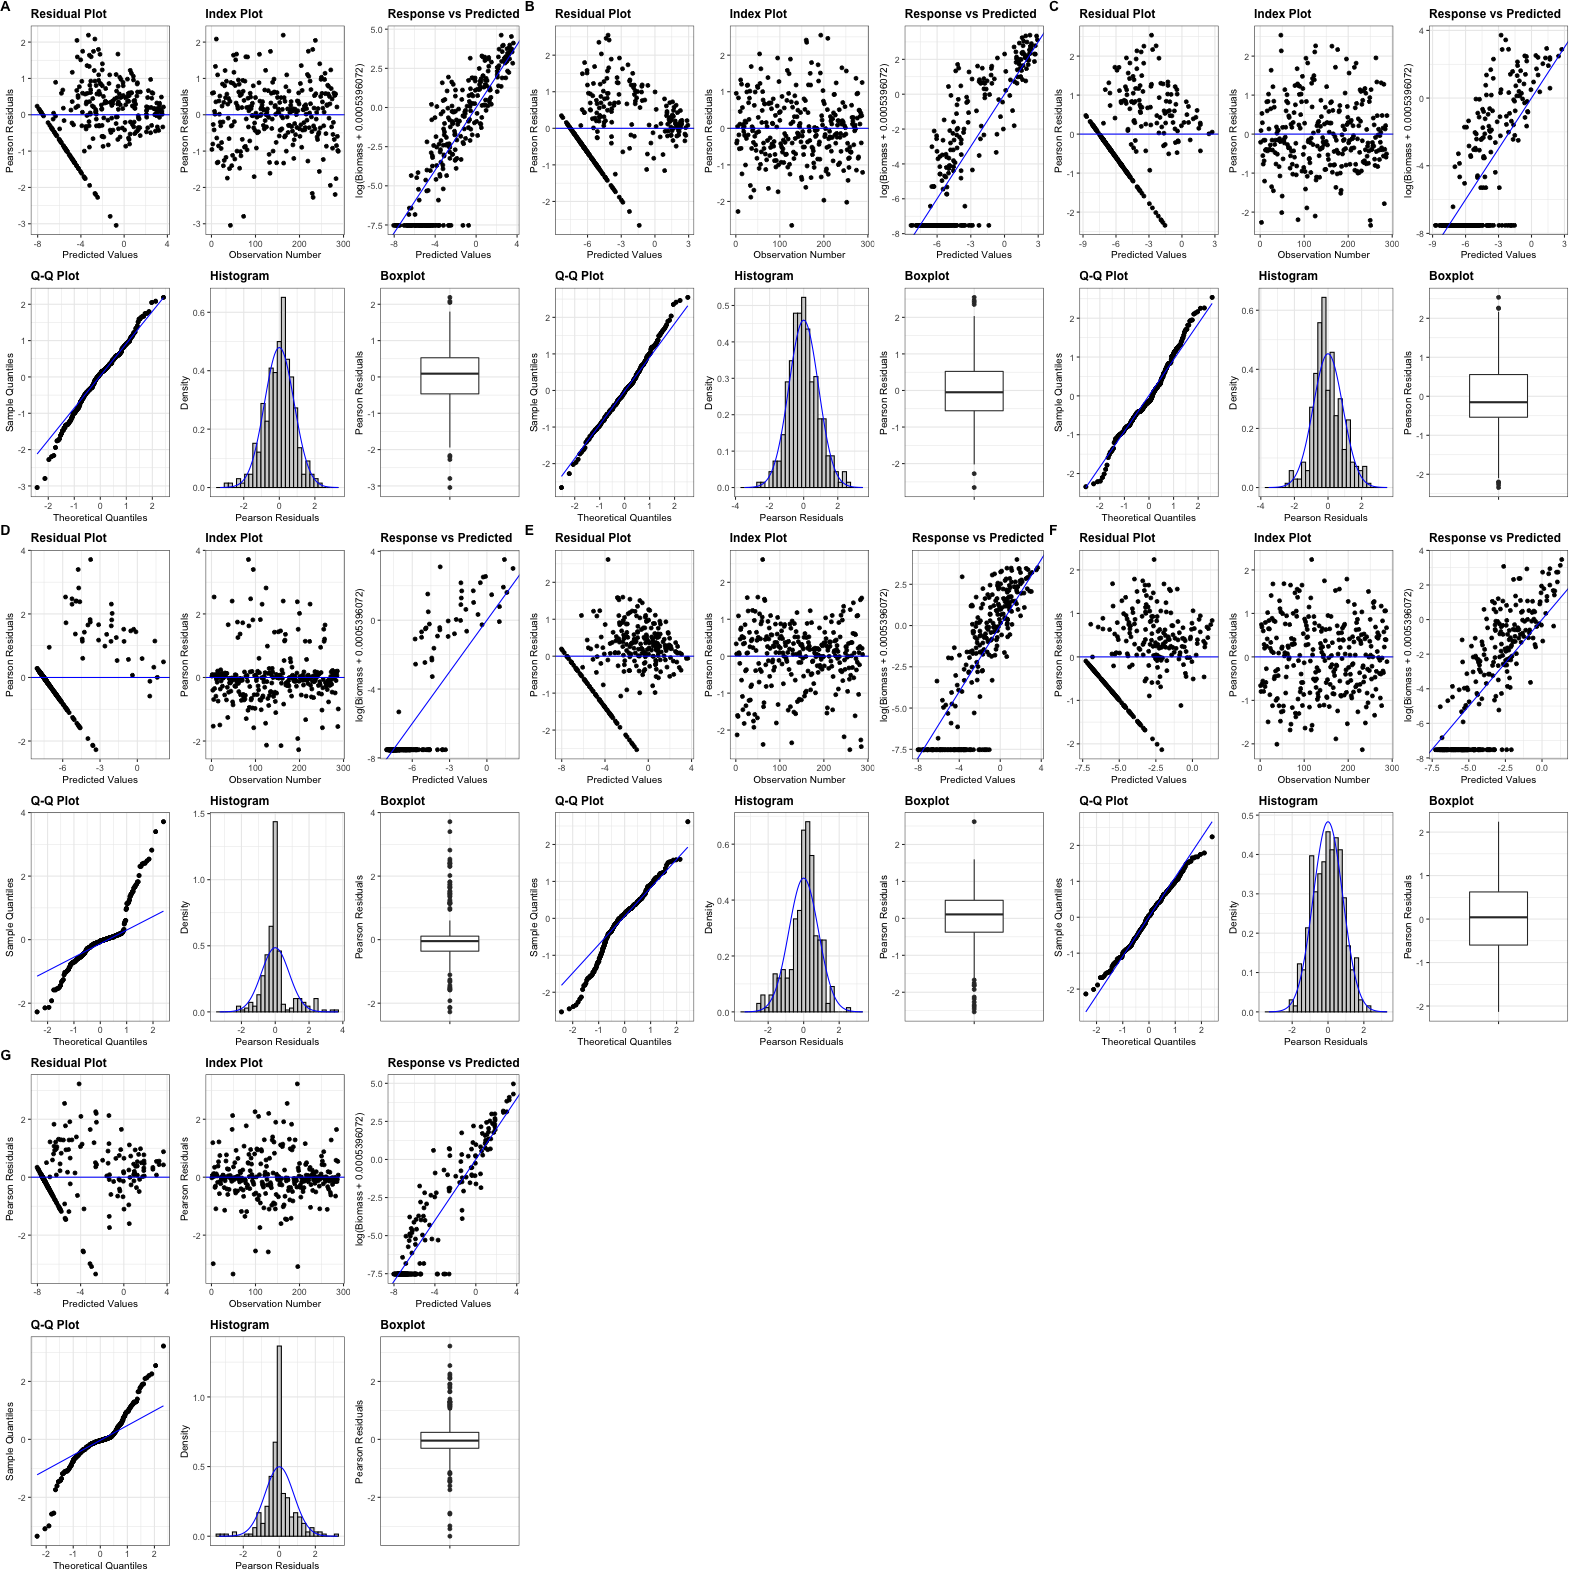
\includegraphics{AppendixA-model-diagnosis_files/figure-latex/sp-biom-diag-1.png}
\caption{\label{fig:sp-biom-diag}Diagnosis plot for the effect of crop identity and corn weed management on the density of (A) - AMATA, (B) - CHEAL, (C) - DIGSA, (D) - ECHCG, (E) - SETFA, (F) - SETLU, and (G) - TAROF}
\end{figure}

\hypertarget{refs}{}
\begin{CSLReferences}{1}{0}
\leavevmode\vadjust pre{\hypertarget{ref-goodeGgResidpanelPanelsInteractive2019}{}}%
Goode, Katherine, and Kathleen Rey. 2019. {``{ggResidpanel}: {Panels} and Interactive Versions of Diagnostic Plots Using 'Ggplot2'.''}

\end{CSLReferences}

\end{document}
